\section{Introduction}

Crop recommendations are often communicated as an order: crop \(i\) is more
suitable than crop \(j\), or a predictive model assigns \(i\) the larger yield
potential. Planting is not an order. It is a vector of land commitments made
before prices, yields and operating conditions are fully known. The distinction
becomes consequential when margins co-move in bad years, when a lender caps
working capital, when rotation rules restrict crop shares, when a contract
requires minimum acreage, or when labour and machinery are shared across
crops. A producer can then rationally plant less of the highest-ranked crop
without rejecting the agronomic information contained in the ranking.

This paper studies that event as \emph{crop-ranking reversal}. For a pair with
score \(s_i>s_j\), reversal means \(x_i<x_j\) in the selected optimal acreage
plan. Strong reversal occurs when the top-ranked crop receives less land than
every lower-ranked crop. The question is not whether a ranking alone identifies
acreage. It does not. The scientific question is sharper: under a declared
stochastic crop-planning model, which economic, risk and operational mechanisms
move the optimum across the ranking boundary, where is the resulting
frontier, and when do conventional diversification or additional information
fail to protect the decision?

Three features make this question difficult. First, the score must remain
conceptually distinct from profit. A revenue score relabelled as
``suitability'' would make the comparison circular. We therefore construct a
genuine pre-decision agronomic index from historical state yield relative to
same-year national yield. Expected margin is constructed separately from
price, yield and operating cost. Second, joint downside risk cannot be
recovered from marginal standard deviations or a single rank-correlation
coefficient. Gaussian, Student-\(t\) and Clayton copulas can match Kendall's
\(\tau\) while assigning different mass to joint crop failures. Third, a
solution returned by one linear-programming run may be one point on an optimal
face. A reversal claim must distinguish whether reversal is possible,
universal across the face, or selected by a declared deterministic rule.

We address all three features in one model. Acreage is chosen to maximize
expected profit subject to a loss-CVaR ceiling and a polyhedral operational
set containing land, idle land, crop bounds, budget, rotation, contractual
minimums and shared labour and equipment. The finite-scenario form is a linear
programme. Its Karush--Kuhn--Tucker system includes the free VaR threshold,
scenario excess variables and every operational multiplier. The full system
prevents a local marginal-value identity from being misread as an acreage
ordering.

Our first contribution is an exact but deliberately restricted reversal
characterization. In a fixed-land two-crop problem where the higher-ranked crop
also has the larger expected margin, its optimal share is the right endpoint
of the risk-feasible interval. Reversal occurs if and only if that endpoint is
below one-half of total land. With additional monotonicity on the upper half,
the condition reduces to CVaR at the equal-share allocation exceeding the
risk ceiling. A unique dependence threshold exists only within a named family
when continuity, strict monotonicity and crossing are verified. Without those
conditions the reversal set can be disconnected. This directly repairs
informal arguments that attempt to infer acreage from a ``risk-adjusted margin
gap'' or from a scalar tail-dependence coefficient.

Our second contribution is a full-model experiment calibrated from official
US agricultural series. Kansas corn, soybean and winter wheat provide
\KansasYears{} complete pre-evaluation years. The score order is winter wheat,
soybean, corn, while mean real margins are \(\$\,\MarginWheat\),
\(\$\,\MarginSoy\) and \(\$\,\MarginCorn\) per acre, respectively. In the
registered Student-\(t\) copula stress model, the 95\% loss-CVaR ceiling binds.
The top-ranked winter wheat receives share \PrimaryWheat, less than corn
(\PrimaryCorn) and soybean (\PrimarySoy). Expected profit is
\(\$\,\PrimaryProfit\) per normalized acre and loss-CVaR is
\(\$\,\PrimaryCVaR\). KKT primal, stationarity and complementarity residuals
are below \(6\times10^{-14}\).

The phase diagram is more informative than this one allocation. Across
\PhaseCells{} registered cells spanning three copula families, five
Kendall-\(\tau\) values and eleven risk tolerances, \PhaseReversal{} cells
reverse and \PhaseStrong{} reverse strongly. Two cells contain multiple
optima, no cells are infeasible, and one Clayton path is disconnected on the
registered grid. Historical resampling gives reversal probability
\BootstrapProbability{} with percentile interval
\([\BootstrapProbabilityLow,\BootstrapProbabilityHigh]\). These quantities
are uncertainty diagnostics for the registered structural stress test, not
estimates of farm-level prevalence.

Our third contribution separates diversification diagnostics that are often
conflated. We define failure only when a conventional Gaussian or
mean--variance policy looks diversified under its own variance criterion,
differs from the tail-aware allocation and has worse loss-CVaR under the
declared true law. At matched Kendall's \(\tau=0.25\), Gaussian advice has
Student-\(t\) loss-CVaR \(\$\,\DiversificationGaussianCVaR\), exceeding the
ceiling \(\$\,\DiversificationRiskCeiling\); the tail-aware allocation attains
\(\$\,\DiversificationTailCVaR\). Thus the failure is operational and
executable rather than a rhetorical claim that ``correlation misses tails.''

Finally, we reconstruct the relation between information and flexibility.
The signal is an imperfect pre-plant indication of relative crop-yield
conditions. In one path, flexibility expands the share that can be reallocated
after observing the signal. This produces strict complementarity when the
posterior-optimal acreage plans differ. In a second path, flexibility buffers
the state-dependent yield shock through recourse interpretable as irrigation,
input switching or harvest timing. There, the information value necessarily
falls to zero when the predicted state is fully buffered, producing
substitution. The registered grid contains \InfoStrictCells{} strict,
\InfoSubCells{} substitutive, \InfoZeroCells{} zero and \InfoBoundaryCells{}
boundary cells.

Figure~\ref{fig:architecture} summarizes the architecture. It preserves the
original scientific chain from suitability to stochastic operational
optimality: score, uncertain margin, joint law, operational set, downside-risk
constraint, reversal frontier, diversification failure and information
actionability. The paper does not recast the topic as a general essay about
ordinal insufficiency. Ordinality is a boundary condition; the contribution
is the conditional mechanism and its verified consequences.

\begin{figure}[t]
\centering
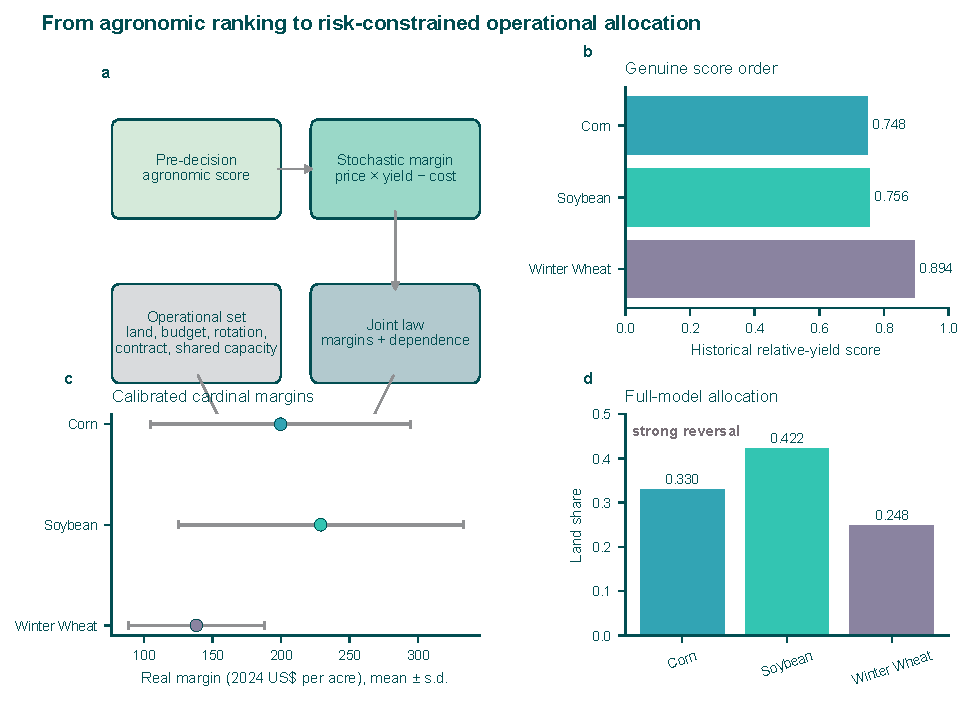
\includegraphics[width=\textwidth]{figures/issue34/Figure1.pdf}
\caption{\textbf{From agronomic ranking to risk-constrained operational
allocation.} \textbf{a}, The score remains external to the profit objective.
Stochastic margins and their joint law enter expected profit and loss-CVaR,
whereas land, budget, rotation, contract and shared-capacity restrictions
define feasible action. \textbf{b}, The pre-decision score ranks winter wheat
first. \textbf{c}, Cardinal mean margins are estimated separately; bars show
one standard deviation across the eight calibration years. \textbf{d}, The
registered full-model optimum assigns the least land to winter wheat and
therefore strongly reverses the score order.}
\label{fig:architecture}
\end{figure}
